\section{The cost--quality frontier}
\label{sec:results}

\begin{figure}[t]
\centering
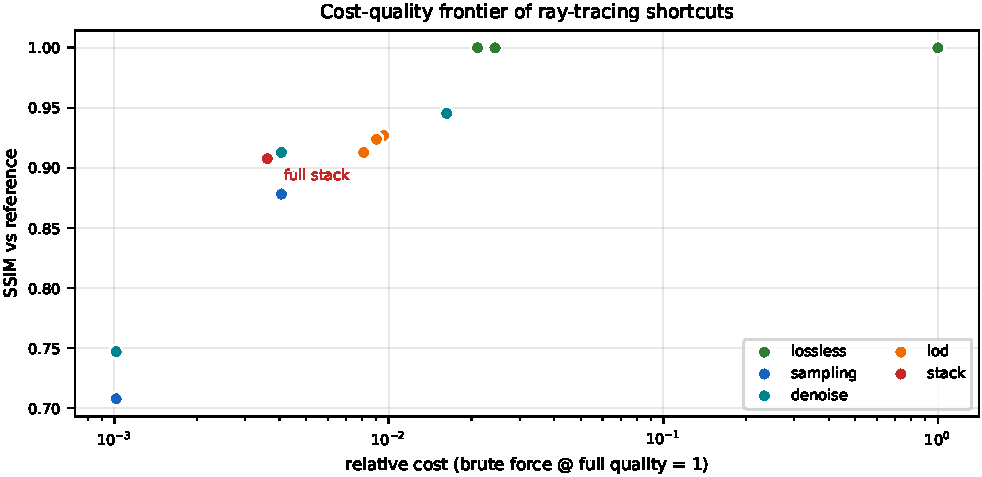
\includegraphics[width=\columnwidth]{figures/pareto.pdf}
\caption{Every technique on one plane: relative cost (log scale, brute force at
full quality $=1$) versus SSIM against the reference. Lossless methods sit at
SSIM $1$ and move left for free; lossy methods trade quality for another order
of magnitude of cost. The full stack combines instancing, LOD, few samples, and
denoising.}
\label{fig:pareto}
\end{figure}

Figure~\ref{fig:pareto} collects the whole study on a single cost--quality
plane. Three things stand out.

First, the two lossless methods are a vertical wall at SSIM $=1$: they buy
\BvhSpeedupRender--\InstSpeedupRender$\times$ (rising with scene size) at zero
quality loss. Any renderer should take this before considering anything else; a
BVH takes brute force from relative cost $1$ to \BvhRelCostPct\% of it with an
identical picture.

Second, the lossy methods extend the frontier by another order of magnitude but
now bend downward in quality. The sample-budget points trace the Monte-Carlo
curve; the denoised points sit above them at equal cost, pushing the frontier up
and to the left. LOD points, by contrast, sit in an awkward region: on this scene,
with a BVH already in place, they save little cost for their quality cost, so
they are Pareto-dominated by simply rendering fewer samples and denoising. This
is scene- and renderer-specific --- LOD earns its keep when geometry, not
sampling, is the bottleneck --- but it is a concrete reminder that a technique's
value depends on what else is already switched on.

Third, the methods compose. The full stack --- instancing for memory, LOD
geometry, four samples per pixel, and the guided denoiser --- reaches SSIM
\StackSsim\ at \StackSpeedup$\times$ less cost than the brute-force reference.
Most of that factor comes from the free, lossless layers; the lossy layers
contribute the last stretch at a quality cost one can see on the plot and decide
whether to pay.

The practical reading is a priority order. Structure first (BVH, instancing):
free, always worth it, and the larger the scene the larger the win. Then spend
the sampling budget where it matters and lean on a geometry-guided denoiser to
stretch it. Reach for LOD when the geometry --- not the noise --- is what is
actually costing you. The ``opportunity cost'' the introduction asked about is,
in the end, legible: it is the vertical drop on Figure~\ref{fig:pareto} you
accept in exchange for each horizontal step left.
